\documentclass{ctexart}
% 全部宏包统一前置，禁止插在document内部
\usepackage{graphicx}
\graphicspath{{./}} % 图片搜索路径，和tex同目录
\usepackage{lastpage}
\usepackage{listings}
\usepackage{xcolor}
\usepackage{float}
\usepackage{amsmath,amssymb}
\usepackage{geometry}
\usepackage{fancyhdr}

% 页面设置
\geometry{a4paper,margin=2cm}
\pagestyle{fancy}
\fancyhf{}
\cfoot{第 \thepage 页 (共\pageref{LastPage}页)}
\setlength{\headheight}{15pt}

% 代码块中文兼容配置
\lstset{
  inputencoding=utf8,
  extendedchars=true,
  basicstyle=\ttfamily\small,
  commentstyle=\color{gray}
}

\begin{document}
% 封面必须放在document内部，之前放在导言区是语法错误
\begin{titlepage}
    \centering

    \vspace*{2cm}

    {\heiti\zihao{2} 信息科学技术学院\par}

    \vspace{0.8cm}

    {\heiti\zihao{3} 课程（实习）设计\par}

    \vspace{2cm}

    \renewcommand{\arraystretch}{2.2}

    \begin{tabular}{rl}
        课程设计名称： & 数据结构课程设计 \\[0.4cm]
        专\qquad\quad 业： & 计算机科学与技术 \\[0.4cm]
        学\qquad\quad 号： & \underline{\hspace{6cm}} \\[0.4cm]
        学 生 姓 名： & \underline{\hspace{6cm}} \\[0.4cm]
        成\qquad\quad 绩： & \underline{\hspace{6cm}} \\[0.4cm]
        批改日期： & \underline{\hspace{6cm}} \\[0.4cm]
        指导教师： & \underline{\hspace{6cm}}
    \end{tabular}

    \vfill

    \today
\end{titlepage}

\maketitle
\tableofcontents
\newpage
\section{模块一}
\subsection{1. 约瑟夫问题}
\subsubsection{任务}
一堆猴子都有编号，编号是 $1,2,3 \dots n$，这群猴子（$n$ 个）按照 $1 \sim n$ 的顺序围坐一圈，从第 $1$ 只开始数，每数到第 $m$ 个，该猴子就要离开此圈，这样依次下来，直到圈中只剩下最后一只猴子，则该猴子为大王。请设计算法编写程序，输出成为大王的猴子的编号。

\subsubsection{（1）需求分析}
\paragraph{分析总结逻辑结构}
本质上是线性结构上的循环删除操作。
\begin{enumerate}
    \item 初始有 $n$ 只猴子，按顺序围成一圈；
    \item 从第 $1$ 只开始按顺时针顺序报数；
    \item 每报到第 $m$ 只猴子，该猴子执行出圈（删除操作）；
    \item 剩余猴子继续顺时针循环报数；
    \item 持续循环，直至圈内仅剩余 $1$ 只猴子，该猴子即为最终大王。
\end{enumerate}

\paragraph{逻辑结果}
\begin{itemize}
    \item 数据之间具备线性邻接关系；
    \item 逻辑上构成环状结构；
    \item 核心操作：循环遍历、删除当前节点。
\end{itemize}

\paragraph{分析总结运算集合}
遍历、计数、标记删除、循环跳转、判停（剩余元素数量为1）。

\subsubsection{（2）概要设计}
\paragraph{存储结构设计}
本问题采用两种存储结构分别实现：

\subparagraph{（1）顺序结构设计}
采用一维顺序表模拟环形结构：
\begin{itemize}
    \item \texttt{int a[N]}：存储猴子编号（取值 $1 \sim n$）；
    \item \texttt{int st[N]}：状态标记数组；
    \item $\texttt{st}[i] = 0$：表示猴子未出圈；
    \item $\texttt{st}[i] = 1$：表示猴子已出圈；
    \item 通过取模运算 $\texttt{(index + 1) \% n}$ 实现环形循环访问。
\end{itemize}

特点：
\begin{itemize}
    \item 结构简单，逻辑直观、易于理解；
    \item 依赖辅助标记顺序表模拟删除；
    \item 时间复杂度较高，需要反复遍历跳过已出圈元素。
\end{itemize}

\subparagraph{（2）链式结构设计}
采用循环单链表表示约瑟夫环：

结构特点：
\begin{itemize}
    \item 每个链表结点存储一只猴子的编号；
    \item 链表尾结点指向头结点，形成闭环循环链表；
    \item 通过指针循环移动完成报数计数；
    \item 修改指针指向完成结点删除操作。
\end{itemize}

优势：
\begin{itemize}
    \item 存储模型贴合约瑟夫环环形问题本质；
    \item 找到目标结点后删除操作时间复杂度 $O(1)$；
    \item 无需额外辅助标记顺序表。
\end{itemize}

\subsubsection{（3）算法设计（流程图）}
本问题分别给出顺序表模拟、循环单链表两种实现思路流程图，下面插入流程图图片。

% 插入图片语法说明
% width=0.8\textwidth：图片占文本宽度80%，可自行修改
% fig1.png 替换为你Overleaf里上传的流程图文件名
\begin{figure}[H]
    \centering
    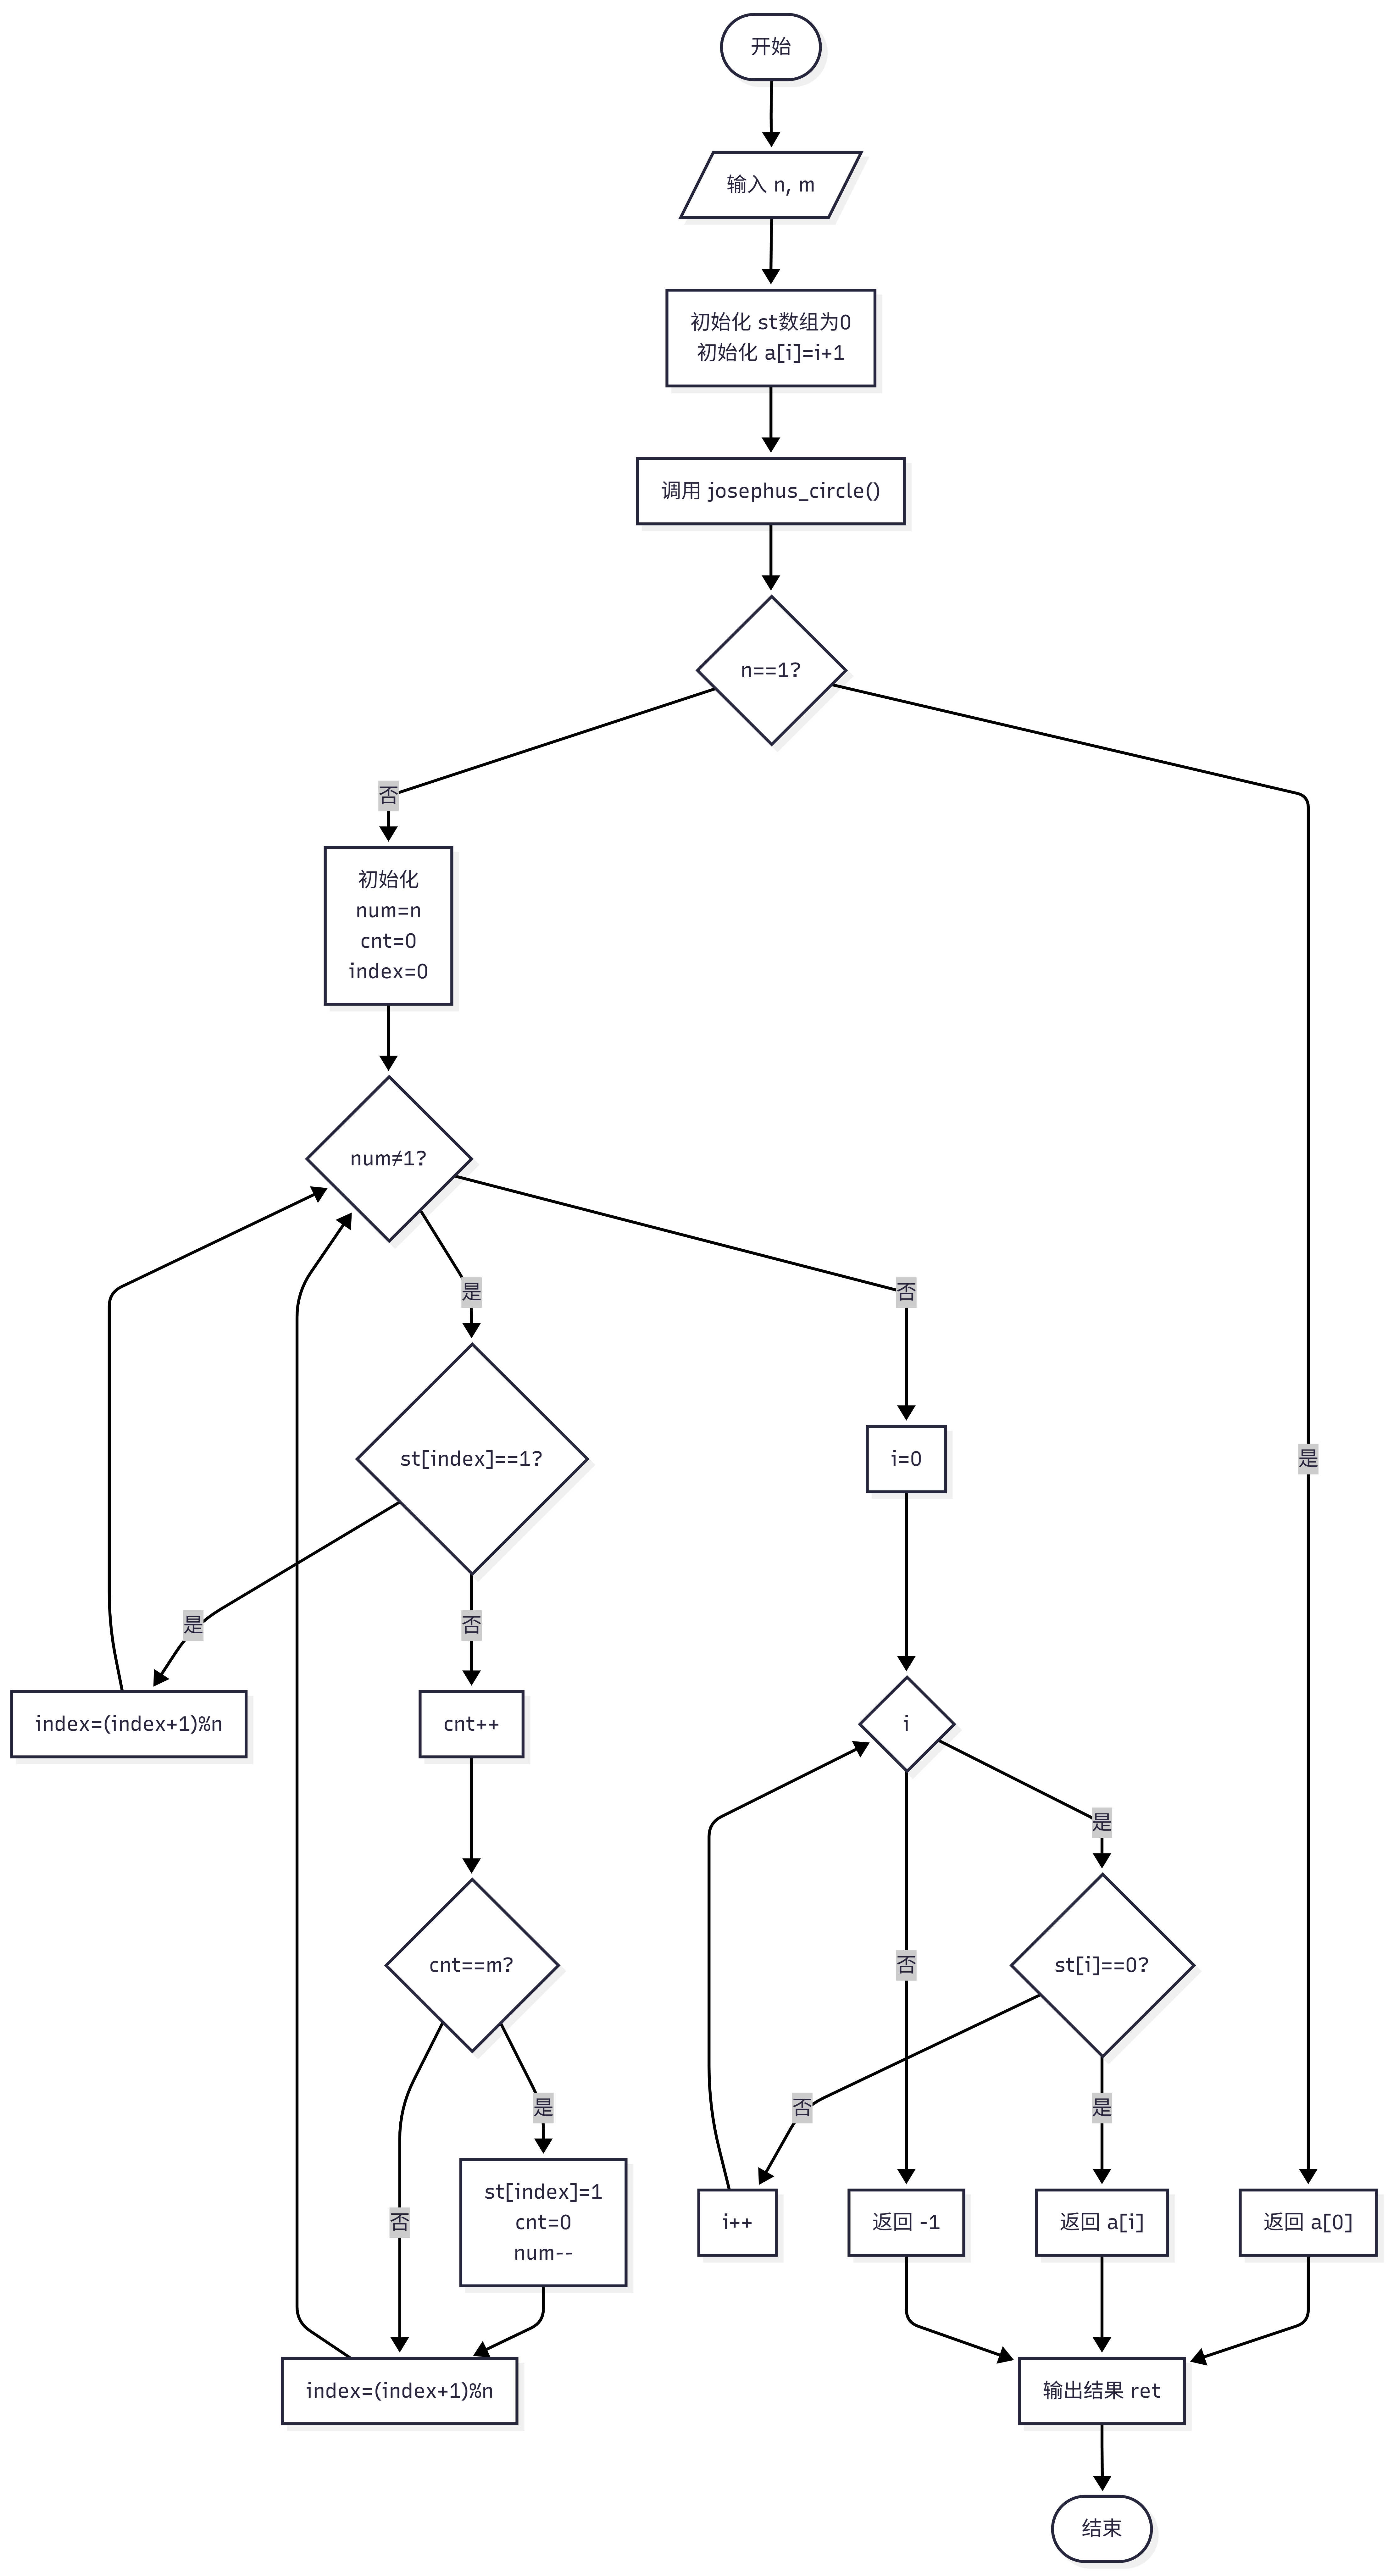
\includegraphics[width=0.8\textwidth]{JosephusProblem_list.png}
    \caption{顺序表模拟约瑟夫环算法流程图}
    \label{fig:joseph-array}
\end{figure}

\subsubsection{（4）详细设计}
\paragraph{源代码（带注释）}
采用 \textbf{左右双栏并排} 展示两种实现代码，左侧为顺序表模拟，右侧为循环单链表实现，阅读顺序为先左后右。

\subsubsection{顺序存储结构实现}

\begin{lstlisting}[caption={顺序表模拟约瑟夫环}]
#include<stdio.h>
#include<stdlib.h>
#include<string.h>

#define N 10000

int a[N], n, m;
int st[N];

int josephus_circle()
{
    // 如果只有一个人
    if (n == 1)
        return a[0];

    int num = n;
    int cnt = 0;
    int index = 0;

    while (num != 1)
    {
        // 已出圈则跳过
        if (st[index] == 1)
        {
            index = (index + 1) % n;
            continue;
        }

        cnt++;

        // 数到第m个
        if (cnt == m)
        {
            st[index] = 1;
            cnt = 0;
            num--;
        }

        index = (index + 1) % n;
    }

    // 找最后剩余的人
    for (int i = 0; i < n; i++)
    {
        if (st[i] == 0)
            return a[i];
    }

    return -1;
}

int main()
{
    printf("请输入n和m：");

    scanf("%d%d", &n, &m);

    memset(st, 0, sizeof(st));

    for (int i = 0; i < n; i++)
        a[i] = i + 1;

    int ret = josephus_circle();

    printf("最后的大王编号为：%d\n", ret);

    return 0;
}
\end{lstlisting}

\subsubsection{使用链式储存解决问题}

\begin{lstlisting}[caption={链式存储模拟约瑟夫环}]
#include<stdio.h>
#include<stdlib.h>

typedef struct node
{
    int data;
    struct node* next;
}node, * list;

//创建一个循环链表，里面有n个节点，节点的data是1到n
list create(int n)
{
    //如果只有一个人，则直接返回一个节点
    if (n == 1)
    {
        node* head = (node*)malloc(sizeof(node));
        head->data = 1;
        head->next = head;
        return head;
    }
    //如果有多个人，则创建一个循环链表
    node* head = NULL;
    node* tail = NULL;
    head = (node*)malloc(sizeof(node));
    tail = (node*)malloc(sizeof(node));
    head->data = 1;
    head->next = tail;
    tail->data = n;
    tail->next = head;
    //从n-1开始，使用头插法创建一个循环链表
    for (int i = n - 1; i >= 2; i--)
    {
        node* t = (node*)malloc(sizeof(node));
        t->data = i;
        t->next = head->next;
        head->next = t;
    }
    return head;
}

int josephus_circle(list head, int m)
{
    node* p = head;
    node* pre = p;
    //直接找到链表的尾结点
    while (pre->next != p)
        pre = pre->next;
    while(p != p->next)
    {
        for (int i = 1; i < m; i++)
        {
            pre = p;
            p = p->next;
        }
        //当数到第m个时，该节点删除
        pre->next = p->next;
        node* tmp = p;
        p = p->next;
        free(tmp);
    }
    int ret = p->data;
    free(p);
    return ret;
}

int main()
{
    int n, m;
    scanf("%d %d", &n, &m);
    node* head = create(n);
    int ret = josephus_circle(head, m);
    printf("%d", ret);
    return 0;
}

\end{lstlisting}

\subsubsection{（5）调试分析}

\paragraph{测试用例1：输入 $n=10,\ m=4$}
运行程序，输入数据：
\begin{verbatim}
请输入n和m：10 4
最后的大王编号为：5
\end{verbatim}
两种存储结构代码运行输出结果一致，结果正确。

\paragraph{测试用例2：输入 $n=6,\ m=6$}
运行程序，输入数据：
\begin{verbatim}
请输入n和m：6 6
最后的大王编号为：4
\end{verbatim}
顺序表实现与循环链表实现输出完全相同，验证算法逻辑无偏差。

\paragraph{调试过程遇到的问题与解决}
\begin{enumerate}
    \item 顺序表模拟时下标越界问题：利用取模运算 \texttt{index = (index + 1) \% n} 实现环形循环访问，限制下标范围在 $0 \sim n-1$，消除越界报错。
    \item 循环链表删除节点内存泄漏：每次出圈节点使用 \texttt{free()} 释放堆内存，程序结束释放最后剩余节点，避免内存泄露。
    \item 链表初始首尾指针定位错误：提前用 \texttt{pre} 指向尾节点，保证删除操作时能正常断开目标节点，防止链表断链。
    \item 边界 $n=1$ 特殊情况处理：单独分支判定，直接返回唯一猴子编号，规避循环逻辑异常。
\end{enumerate}

\subsubsection{（6）小结}
本次实验分别采用顺序表、循环单链表两种存储结构完成约瑟夫环问题求解。顺序表模拟实现代码简洁易懂，无需复杂指针操作，但需要额外标记顺序表记录出圈状态，存在大量无效遍历，时间效率偏低；循环链表模型贴合约瑟夫环环形结构本质，节点删除仅修改指针，删除操作效率更高，无需辅助标记顺序表，但涉及动态内存分配、指针移动与内存释放，代码逻辑更复杂。

通过两套方案对比实现，直观区分了顺序存储与链式存储在环形删除场景下的优劣，加深了对线性表、循环链表逻辑结构与基础操作的实操理解，同时掌握了边界测试、内存管理、下标循环等程序调试技巧.


\subsection{2. 纸牌游戏}
\subsubsection{任务}
编号为 1-52 张牌，正面向上，从第 2 张开始，以 2 为基数，是 2 的倍数的牌翻一次，直到最后一张牌；然后，从第 3 张开始，以 3 为基数，是 3 的倍数的牌翻一次，直到最后一张牌；然后从第 4 张开始，以 4 为基数，是 4 的倍数的牌翻一次，直到最后一张牌；……直到以 52 为基数的牌翻过，这时正面向上的牌有哪些？请设计算法编写程序输出最终正面向上的纸牌的编号。

\subsubsection{（1）需求分析}
\paragraph{分析总结逻辑结构}
本题涉及的核心数据对象为：卡牌集合 $\text{Card} = \{1, 2, 3, \dots, 52\}$
每张卡牌有一个状态：
\begin{itemize}
    \item $0$：正面
    \item $1$：反面
\end{itemize}
本题涉及的主要运算：
\begin{enumerate}
    \item 初始化操作：将所有卡牌状态初始化为 $0$；
    \item 状态翻转操作：$\texttt{card[j] = card[j] \textasciicircum 1}$，实现 $0 \leftrightarrow 1$ 状态切换；
    \item 循环遍历操作：外层控制步长 $i$（$2 \sim 52$），内层按 $i$ 间隔访问 $j$（$j = i,2i,3i\dots$）；
    \item 判定输出操作：遍历数组，输出满足 $\texttt{card[i] == 0}$ 的卡牌编号。
\end{enumerate}

\paragraph{分析总结运算集合}
基于顺序线性结构，双层循环模拟完整翻牌流程，包含初始化、倍数遍历、状态翻转、结果筛选输出四类基础运算。

\subsubsection{（2）概要设计}
\paragraph{存储结构设计}
采用一维顺序数组存储卡牌状态：
\begin{itemize}
    \item 数组下标对应卡牌编号 $1 \sim 52$；
    \item 数组元素值记录卡牌状态：$0$ 代表正面，$1$ 代表反面；
    \item 数组长度设置为 $60$，预留多余下标空间，简化边界判断，避免下标越界问题。
\end{itemize}

\paragraph{算法设计思路}
提供两种实现方案：
1. 暴力模拟法：双层循环完整复刻题目翻牌规则，直观还原操作流程；
2. 数学规律法：利用约数成对出现、完全平方数约数个数为奇数的数学特性，直接求解结果，省去多层循环。

\subsubsection{（3）详细设计}
\paragraph{源代码（带注释）}

\begin{figure}[H]
    \centering
    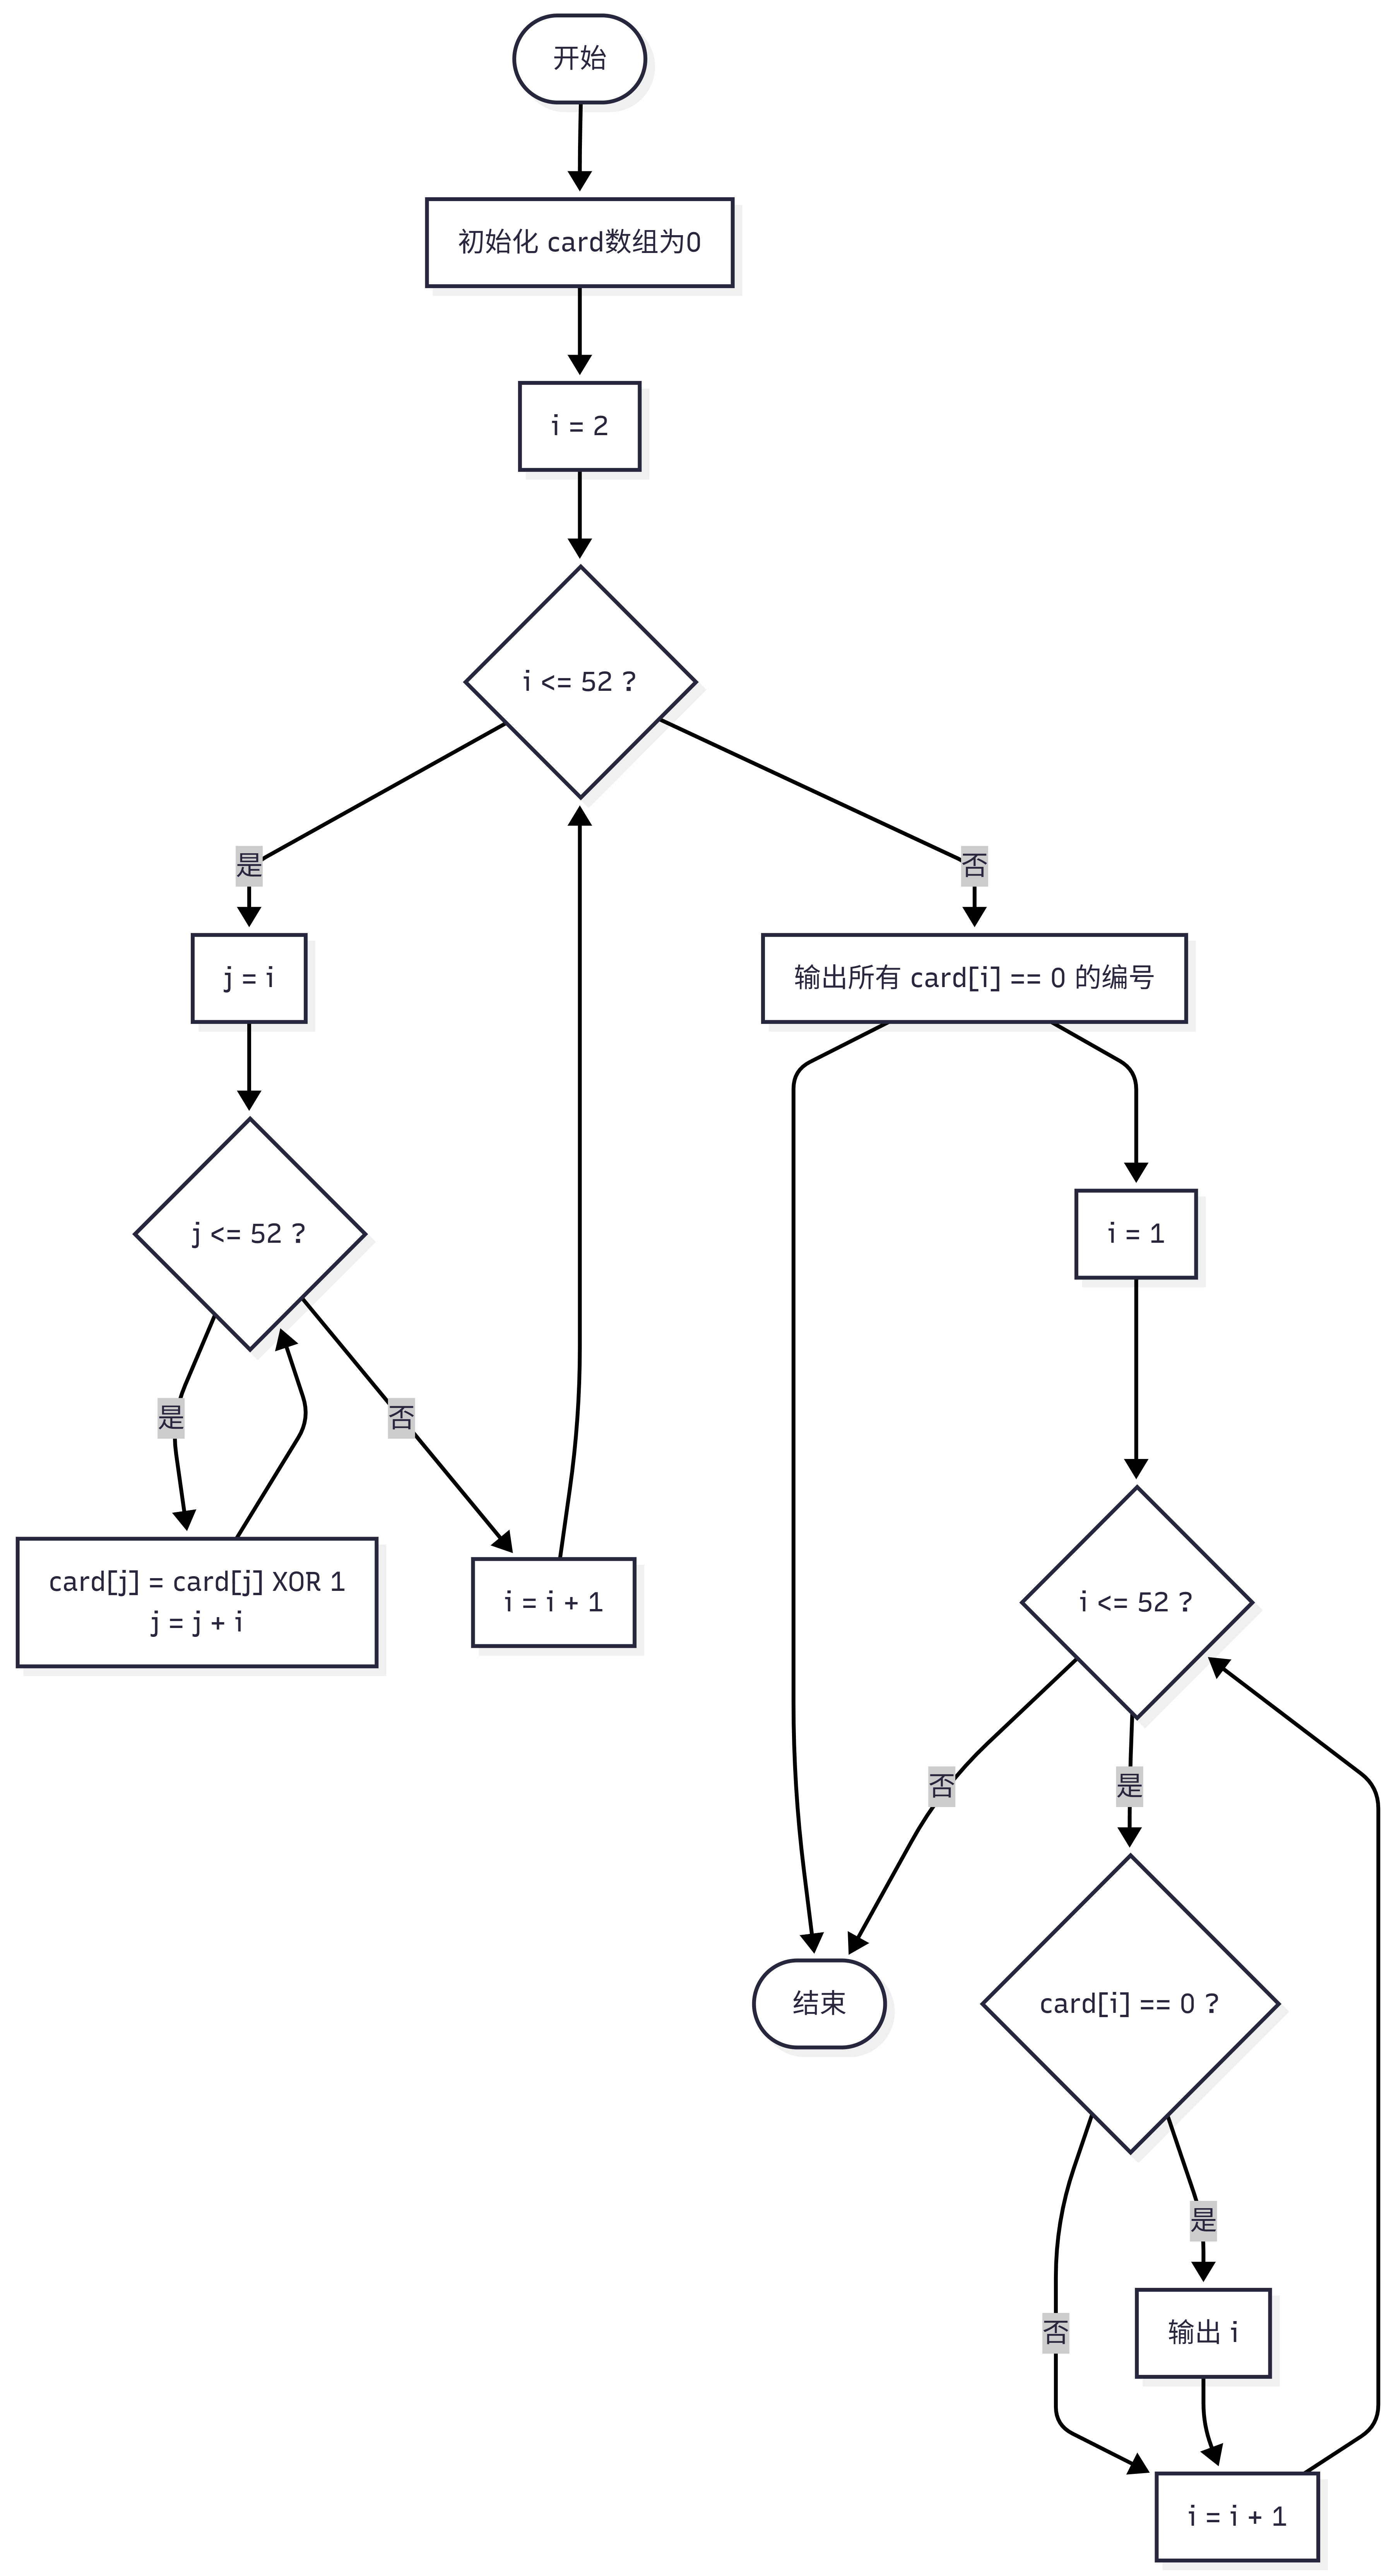
\includegraphics[width=0.8\textwidth]{CardGame-2026-06-23-011504.png}
    \caption{纸牌翻转程序}
    \label{fig:joseph-array}
\end{figure}

\subsubsection{方法一：暴力模拟实现}
\begin{lstlisting}[caption={暴力模拟纸牌翻转程序}]
#include<stdio.h>

int card[60] = { 0 };
//0表示正面，1表示反面
int main()
{
    //从第二张卡牌开始，以i为基数，反转卡牌
    for (int i = 2; i <= 52; i++)
    {
        //从第i张卡牌开始，每隔i张卡牌反转一次
        for (int j = i; j <= 52; j += i)
        {
            card[j] = card[j] ^ 1;
        }
    }
    for (int i = 1; i <= 52; i++)
    {
        //如果卡牌是正面，则输出卡牌编号
        if (card[i] == 0)
            printf("%d ", i);
    }
    return 0;
}
\end{lstlisting}

\subsubsection{方法二：数学规律优化实现}
\begin{lstlisting}[caption={基于完全平方数数学规律求解程序}]
#include<stdio.h>

int card[60] = { 0 };
//可以得出规律，只有完全平方数位置的卡牌才可能是正面
//因为每一个数字的约数都是成双成对存在的，
//但是完全平方数的约数中有一个是重复的，所以完全平方数位置的卡牌被翻开的次数是奇数。
int main()
{
    
    for (int i = 1; i * i <= 52; i++)
    {
        card[i * i] = 1;
    }
    for (int i = 1; i <= 52; i++)
        if (card[i] == 1)
            printf("%d ", i);
    return 0;
}
\end{lstlisting}

\subsubsection{（4）调试分析}
\paragraph{标准测试结果}
程序运行后，最终保持正面向上的纸牌编号输出：
\begin{verbatim}
1 4 9 16 25 49
\end{verbatim}
模拟法与数学规律法输出结果完全一致，验证两种算法逻辑均正确。

\paragraph{调试过程遇到的问题与解决}
\begin{enumerate}
    \item 数组下标从0开始混淆卡牌编号：数组下标1~52与卡牌编号一一对应，舍弃下标0不使用，规避编号错位；
    \item 循环起始边界错误：外层循环基数从2开始，内层翻牌从当前基数卡牌起步，修正循环初始值保证翻牌规则匹配题目要求；
    \item 数学法逻辑颠倒：翻转奇数次为反面、偶数次为正面，完全平方数翻转次数为奇数，对应反面，最终输出正面时筛选非完全平方数，核对逻辑后修正输出判定条件。
\end{enumerate}

\subsubsection{（5）小结}
本次实验采用暴力模拟、数学规律优化两种思路解决纸牌翻转问题。暴力模拟法代码逻辑直观，逐步骤还原翻牌全过程，便于理解题目操作流程，但嵌套循环执行效率偏低；数学规律法依托约数的数学性质，仅通过单层循环遍历完全平方数即可得到答案，代码简洁、运行效率极高。

两种方案对比实现，体会到暴力模拟与数学优化两种编程解题思路的差异，认识到结合数学规律可大幅简化程序逻辑、降低时间复杂度，加深了数学知识与程序算法结合解题的实践认知.


\subsection{3. 一元多项式计算}
\subsubsection{任务}
设计合适的存储结构，完成一元多项式的相关运算。
要求：（1）能够按照指数降序排列建立并输出多项式；（2）能够完成两个多项式的相加、相减，并将结果输出。

\subsubsection{（1）需求分析}
\paragraph{分析总结逻辑结构}
本程序处理对象为一元多项式。每一项由系数和指数两部分组成，因此可将多项式表示为若干项的线性集合。由于需要按照指数降序排列、进行同类项合并以及实现多项式加减运算，采用带头指针的单链表作为存储结构较为合适。
链表中的每个结点表示多项式的一项，结点中包含：
\begin{itemize}
    \item 系数（coef）
    \item 指数（exp）
    \item 指向下一项的指针（next）
\end{itemize}
整个多项式由若干结点按指数递减顺序连接形成，整体逻辑结构属于线性结构。

\paragraph{分析总结运算集合}
多项式创建、按指数降序插入结点、同类项合并、多项式打印、多项式加法、多项式减法、链表内存释放。

\subsubsection{（2）概要设计}
\paragraph{存储结构设计}
采用单链表存储一元多项式，每个节点存储一项的系数与指数，节点按指数从大到小有序排列；插入时自动合并同指数项，系数为0时直接删除节点。
\paragraph{算法设计思路}
1. 插入算法：遍历链表对比指数，找到插入位置，存在同指数则合并系数，系数归零则删除节点；
2. 加法算法：复制两个多项式所有项插入新链表，自动完成同类项合并；
3. 减法算法：复制A多项式，将B多项式各项系数取负后插入新链表，自动合并同类项；
4. 输出算法：对不同指数（0次、1次、高次）做格式化打印，处理正负号、系数±1的特殊显示。

\subsubsection{（3）详细设计}
\paragraph{源代码（带注释）}

\begin{figure}[H]
    \centering

    \begin{minipage}{0.48\textwidth}
        \centering
        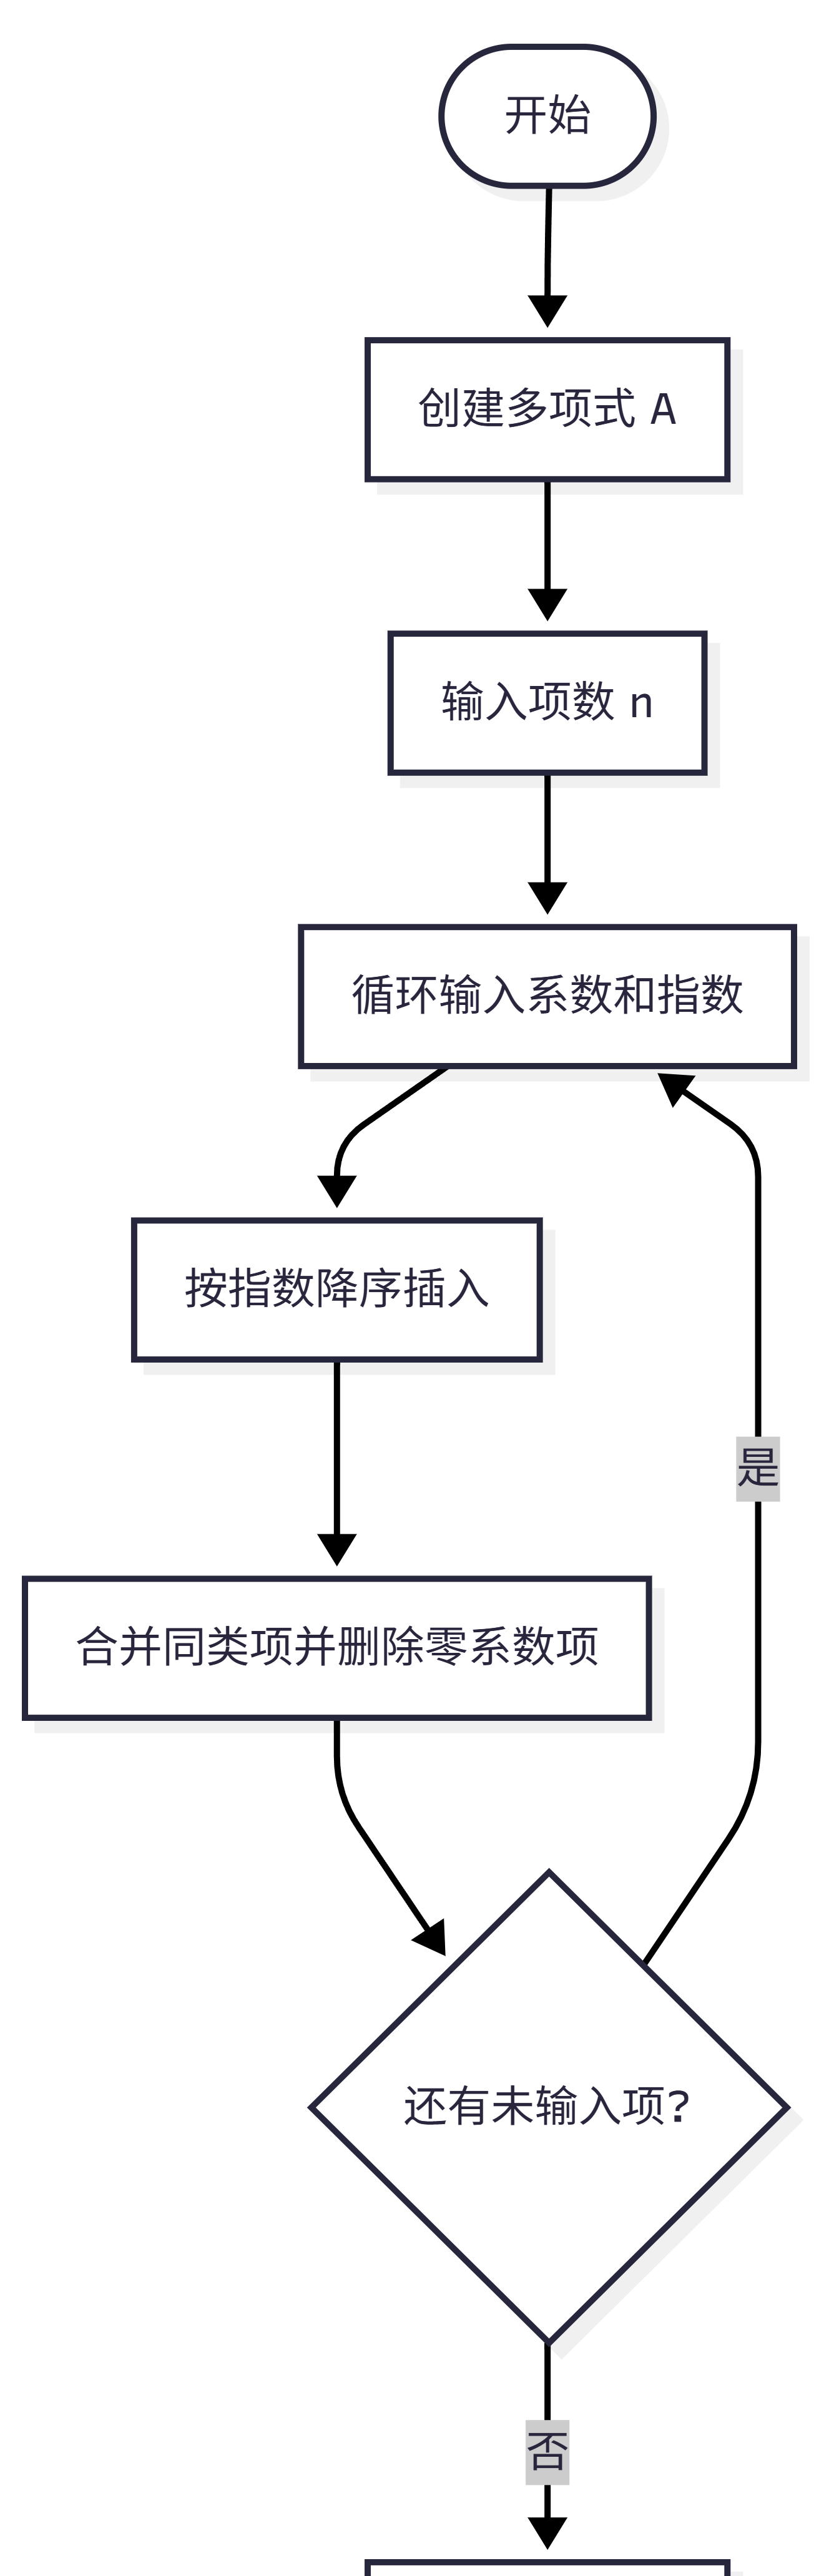
\includegraphics[width=\linewidth]
        {Input Processing Condition-2026-06-23-123520.png}
        \caption{一元多项式计算流程图}
        \label{fig:cardgame}
    \end{minipage}
    \hfill
    \begin{minipage}{0.48\textwidth}
        \centering
        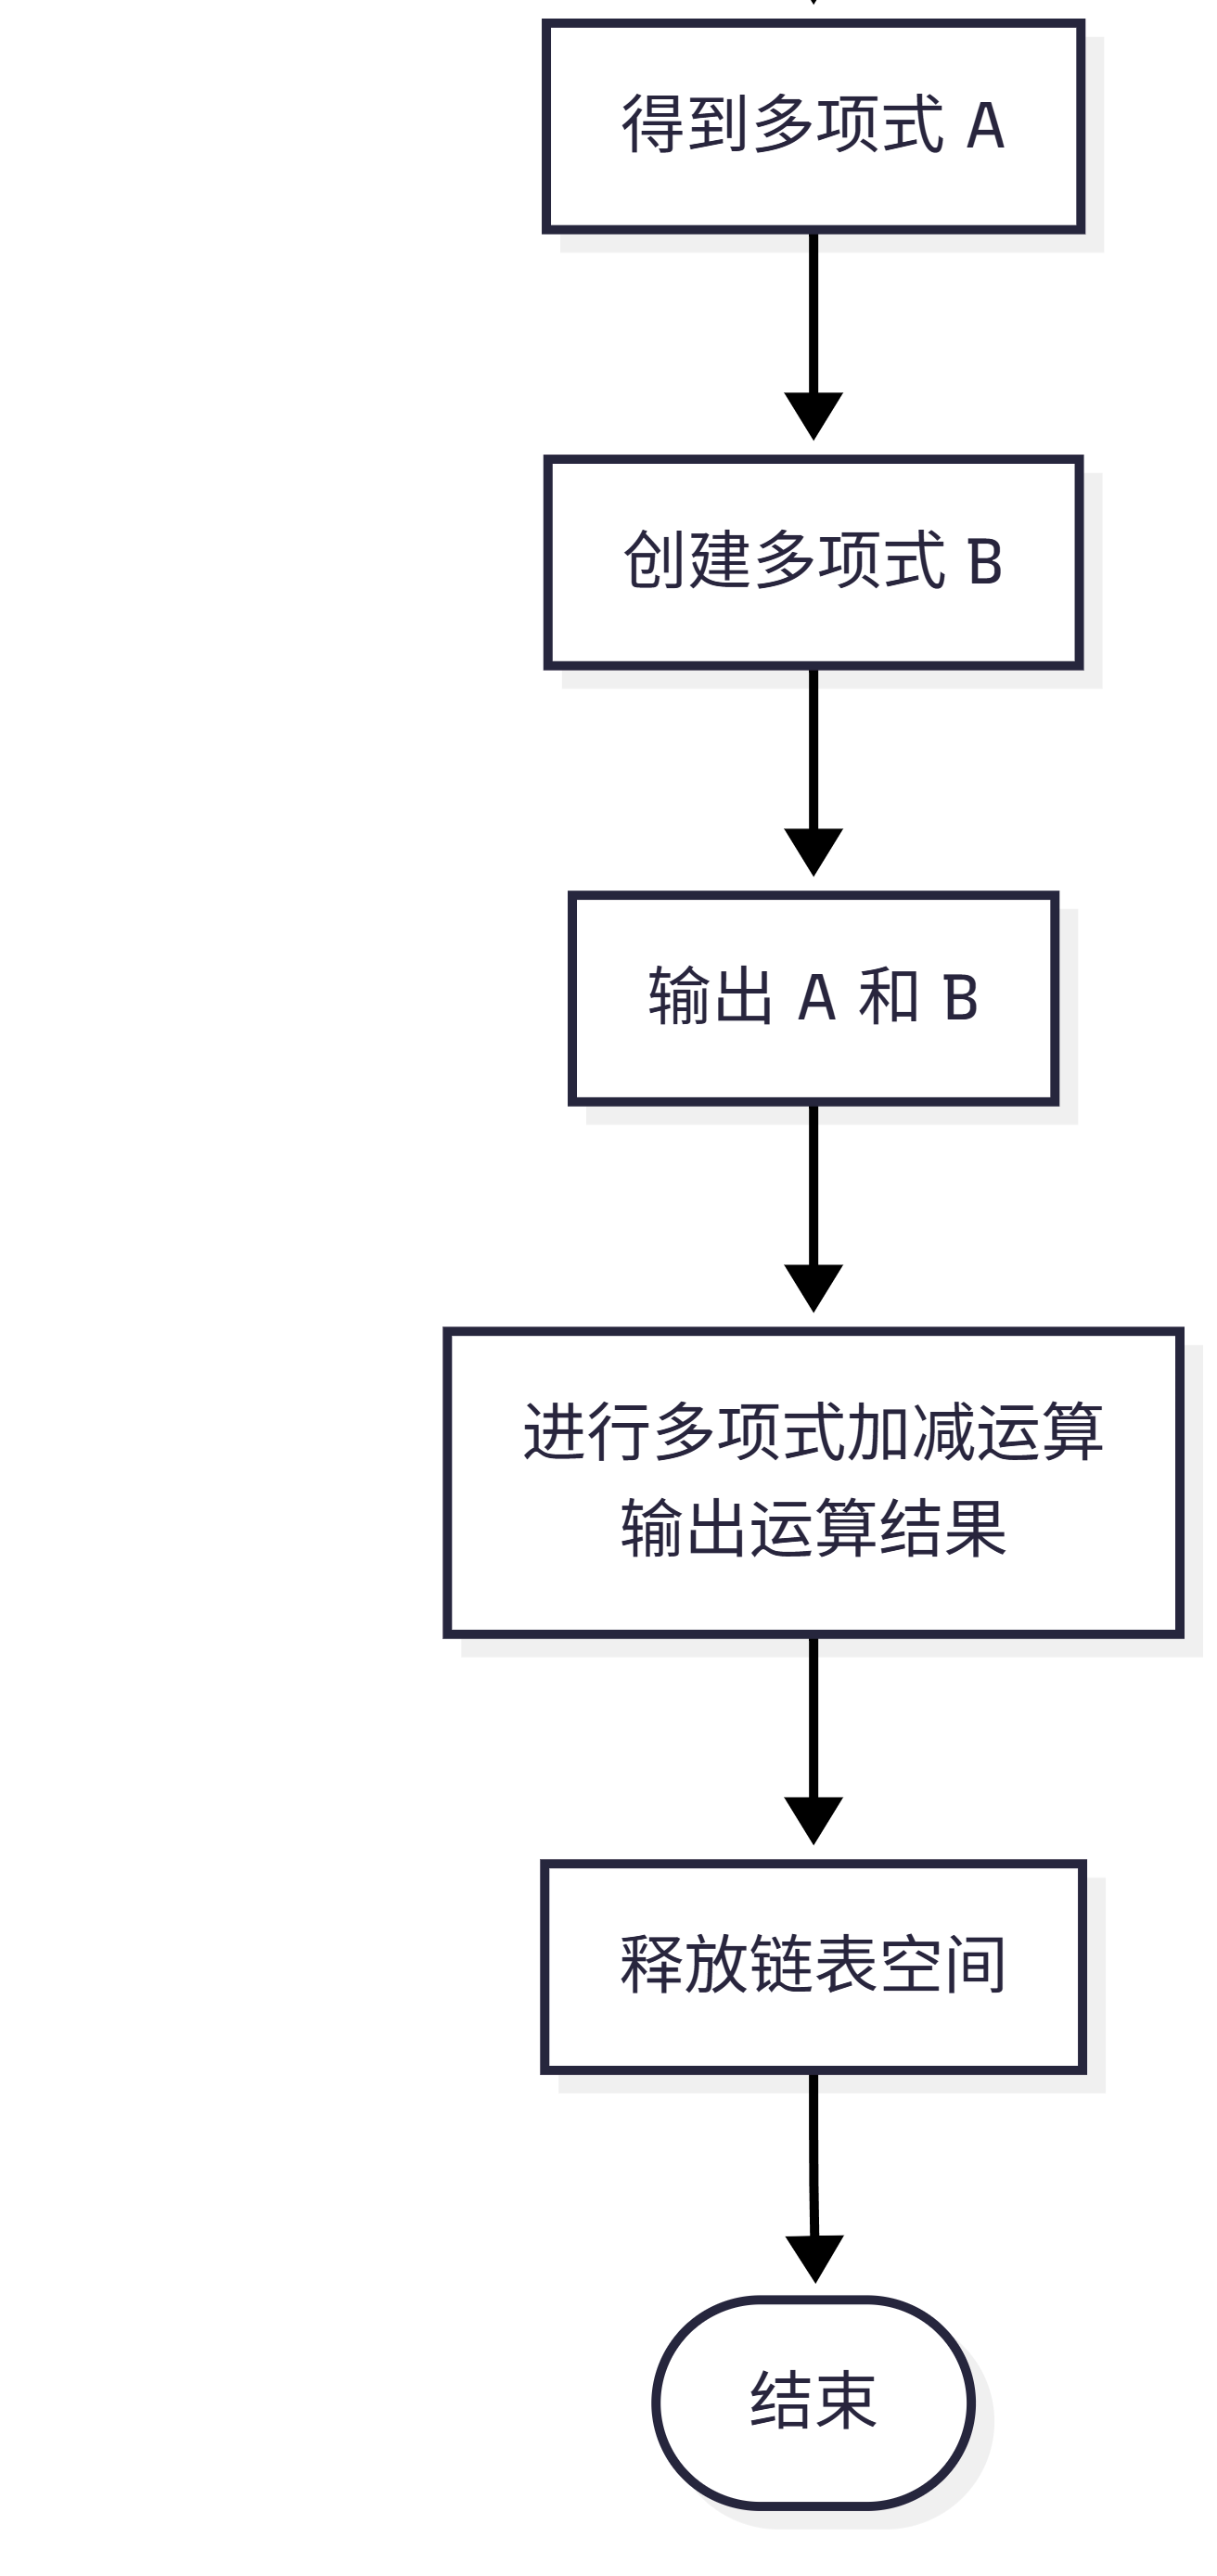
\includegraphics[width=\linewidth]
        {Input Processing Condition-2026-06-23-123520 - 副本2.png}
        \caption{一元多项式计算流程图}
        \label{fig:cardgame-test}
    \end{minipage}

\end{figure}

\begin{lstlisting}[caption={单链表实现一元多项式加减运算}]
// 3． 一元多项式计算
// 任务：设计合适的存储结构，完成一元多项式的相关运算。
// 要求：（1）能够按照指数降序排列建立并输出多项式；（2）能够完成两个多项式的相加、
// 相减，并将结果输出。
#include <stdio.h>
#include <stdlib.h>

typedef struct node
{
    int coef;              // 系数 coefficient
    int exp;               // 指数 exponent
    struct node *next;
}Node, *Polynomial;

// 创建结点
Node *newNode(int coef, int exp)
{
    Node *p = (Node *)malloc(sizeof(Node));
    p->coef = coef;
    p->exp = exp;
    p->next = NULL;
    //返回节点
    return p;
}

// 按指数降序插入
void insert(Polynomial *head, int coef, int exp)
{
    if (coef == 0)
        return;

    Node *p = newNode(coef, exp);

    // 空链表或插入到表头
    if (*head == NULL || (*head)->exp < exp)
    {
        p->next = *head;
        *head = p;
        return;
    }

    Node *pre = NULL;
    Node *cur = *head;

    while (cur && cur->exp > exp)
    {
        pre = cur;
        cur = cur->next;
    }

    // 存在相同指数，合并同类项
    if (cur && cur->exp == exp)
    {
        cur->coef += coef;

        // 系数变成0，删除该项
        if (cur->coef == 0)
        {
            if (pre == NULL)
                *head = cur->next;
            else
                pre->next = cur->next;

            free(cur);
        }

        free(p);
    }
    else
    {
        p->next = cur;

        if (pre == NULL)
            *head = p;
        else
            pre->next = p;
    }
}

// 创建多项式
void create(Polynomial *head)
{
    *head = NULL;

    int n;
    printf("请输入项数：");
    scanf("%d", &n);

    printf("请输入每一项的系数和指数：\n");

    for (int i = 0; i < n; i++)
    {
        int coef, exp;
        scanf("%d%d", &coef, &exp);
        insert(head, coef, exp);
    }
}

// 输出多项式
void printPoly(Polynomial head)
{
    //如果为空，则定义为
    if (head == NULL)
    {
        printf("0\n");
        return;
    }

    Node *p = head;
    int first = 1;

    while (p)
    {
        if (!first && p->coef > 0)
            printf("+");

        if (p->exp == 0)
            printf("%d", p->coef);
        else if (p->exp == 1)
        {
            if (p->coef == 1)
                printf("x");
            else if (p->coef == -1)
                printf("-x");
            else
                printf("%dx", p->coef);
        }
        else
        {
            if (p->coef == 1)
                printf("x^%d", p->exp);
            else if (p->coef == -1)
                printf("-x^%d", p->exp);
            else
                printf("%dx^%d", p->coef, p->exp);
        }

        first = 0;
        p = p->next;
    }

    printf("\n");
}

// 多项式加法
Polynomial add(Polynomial A, Polynomial B)
{
    Polynomial C = NULL;

    Node *p = A;
    while (p)
    {
        insert(&C, p->coef, p->exp);
        p = p->next;
    }

    p = B;
    while (p)
    {
        insert(&C, p->coef, p->exp);
        p = p->next;
    }

    return C;
}

// 多项式减法 A-B
Polynomial subtract(Polynomial A, Polynomial B)
{
    Polynomial C = NULL;

    Node *p = A;
    while (p)
    {
        insert(&C, p->coef, p->exp);
        p = p->next;
    }

    p = B;
    while (p)
    {
        insert(&C, -p->coef, p->exp);
        p = p->next;
    }

    return C;
}

// 释放链表
void destroy(Polynomial head)
{
    Node *p;

    while (head)
    {
        p = head;
        head = head->next;
        free(p);
    }
}

int main()
{
    Polynomial A, B, C, D;

    printf("创建第一个多项式：\n");
    create(&A);

    printf("\n创建第二个多项式：\n");
    create(&B);

    printf("\nA(x) = ");
    printPoly(A);

    printf("B(x) = ");
    printPoly(B);

    C = add(A, B);
    printf("\nA(x)+B(x) = ");
    printPoly(C);

    D = subtract(A, B);
    printf("A(x)-B(x) = ");
    printPoly(D);

    destroy(A);
    destroy(B);
    destroy(C);
    destroy(D);

    return 0;
}
\end{lstlisting}

\subsubsection{（4）调试分析}
\paragraph{测试用例输入与运行结果}
\begin{verbatim}
创建第一个多项式：
请输入项数：4
请输入每一项的系数和指数：
1 3 -1 2 1 1 -3 0

创建第二个多项式：
请输入项数：4 
请输入每一项的系数和指数：
1 3 -1 1 1 0 2 2

A(x) = x^3-x^2+x-3
B(x) = x^3+2x^2-x+1
A(x)+B(x) = 2x^3+x^2-2
A(x)-B(x) = -3x^2+2x-4
\end{verbatim}
两组多项式加减运算输出结果数学计算一致，程序合并同类项、格式化输出逻辑正确。

\paragraph{调试中出现的问题与解决方案}
\begin{enumerate}
    \item 插入多项式时指数乱序：插入函数遍历链表按指数大小寻找插入点，保证链表始终降序排列；
    \item 同指数项未合并：插入时匹配相同指数节点，累加系数，系数归零则释放节点，消除零项；
    \item 打印格式混乱（多余+、1/-1重复输出）：增加first标记区分首项，对指数0、指数1、高次幂分别格式化输出；
    \item 内存泄漏：程序结束调用destroy函数遍历释放所有链表节点，回收堆内存；
    \item 减法逻辑错误：多项式减法等价于A加负B，遍历B时对系数取负再插入结果链表。
\end{enumerate}

\subsubsection{（5）小结}
本次实验使用单链表存储一元多项式，实现多项式有序创建、输出及加减运算，完成同类项合并，掌握链表基础操作，明晰链式存储适配动态数据运算的优势.

\end{document}